\documentclass[10pt,aspectratio=1610]{beamer} % use option aspectratio=169 or 1610 for wide slides
% Note: For online presentations via Zoom use the ratio of the screen you want to share
\usetheme{Rochester}

% load syscop style
\usepackage{style/syscop}

%--------------------------------------------------
% TITLE
%--------------------------------------------------

% NOTE: what's in [ ] goes to footer for the fields title, author and date
\title[Another Short Report on Riccati Solver]{\huge Another Short Report on Riccati Solver}


%--------------------------------------------------
% Useful packages
%--------------------------------------------------

\usepackage{mathtools}
\usepackage{mathdots}
\usepackage{graphicx}
\usepackage{optidef}
\usepackage{booktabs}
\usepackage{diagbox}
\usepackage{multirow}
\usepackage{geometry}
\usepackage{subcaption}
\usepackage{nicematrix}

\begin{document}

\InsertTitle

\begin{frame}
    \frametitle{Quick update}
    Several quick updates on my current progress:
    \begin{itemize}
        \item Expand indefinite QP test cases from Sweet OCP
        \item Try more heuristic methods: Inertial LM from IPOPT and Precompute from Gianluca
        \item Attempt for flop counting
        \item Results: performance profile, geometric mean of cost, flop count
    \end{itemize}
\end{frame}

% Ensure \usepackage{amsmath} is included in your document preamble
\begin{frame}
    \frametitle{test set expansion}
    Thanks David for providing the test set from Sweet OCP \cite{Kiessling2026},
    we extend the cases by modifying the following OCPs:
    \begin{itemize}
        \item acrobot: $\mathrm{n}_x=4 \mathrm{,} \mathrm{n}_u=1$
        \item dubins car parallel parking: $\mathrm{n}_x=3 \mathrm{,} \mathrm{n}_u=2$
        \item dubins car obstacle : $\mathrm{n}_x=3 \mathrm{,} \mathrm{n}_u=2$
        \item flying robot: $\mathrm{n}_x=6 \mathrm{,} \mathrm{n}_u=4$
        \item robot arm: $\mathrm{n}_x=6 \mathrm{,} \mathrm{n}_u=3$
    \end{itemize}
    Total 132 cases now.
\end{frame}

\begin{frame}
    \frametitle{Heuristic methods}
    Inertial correction from IPOPT:
    \begin{figure}[H]
        \centering
        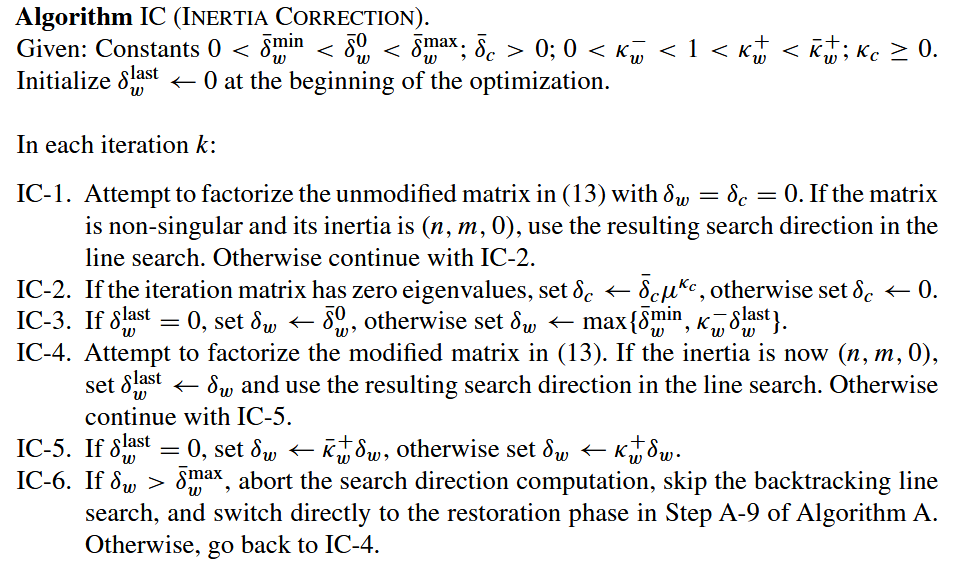
\includegraphics[width=0.60\textwidth]{results/IC.png}
    \end{figure}
    Precompute regularized unmodified Hessian: compute unmodified Hessian at the first iteration, and reuse it for all iterations if Cholesky factorization fails.
\end{frame}

\begin{frame}
    \frametitle{Flop counting}
    In order to estimate the flop counting, we take one modified Cholesky factorization on block reduced Hessian as the unit, i.e.
    \begin{equation*}
        \mathrm{unit} \approx \frac{1}{3} \mathrm{n}_u^3 \mathrm{,}
    \end{equation*}
    where $\mathrm{n}_u$ is the control dimension of the problem.
    \vspace{0.2cm}

    The flops of eigenvalue decomposition is usually regarded as $9n^3$ \cite{verschuerenTimeoptimalRaceCar2016b}, 
    which is 27 units if modifying the block reduced Hessian.
\end{frame}

\begin{frame}
    \frametitle{Results: performance profile}
    \begin{figure}[H]
        \centering
        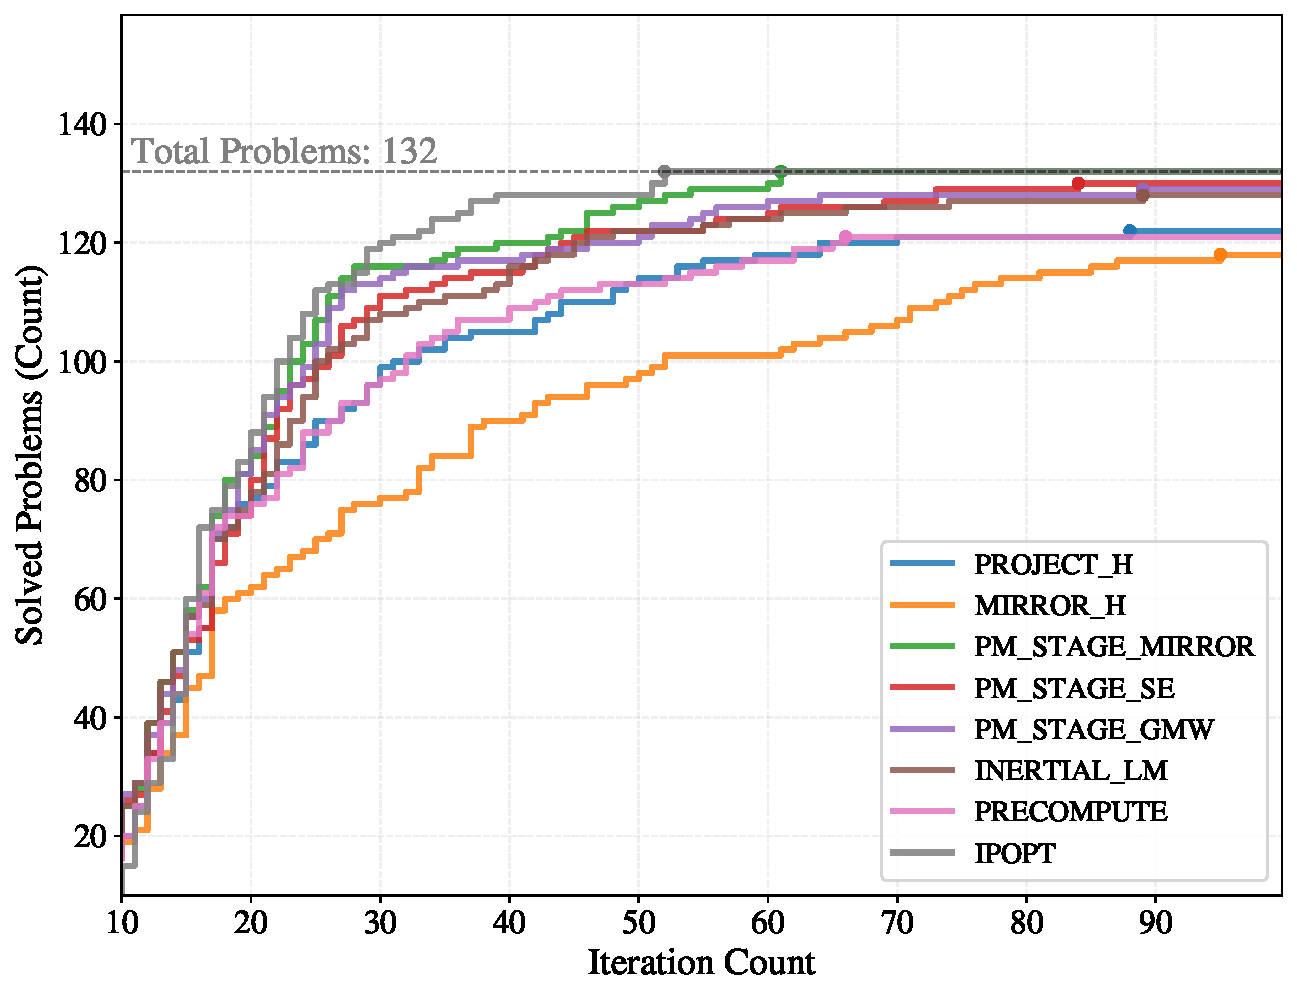
\includegraphics[width=0.70\textwidth]{results/iteration_qp_results_riccati.pdf}
    \end{figure}
\end{frame}

\begin{frame}
    \frametitle{Results: geometric mean of cost}
    \begin{figure}[H]
        \centering
        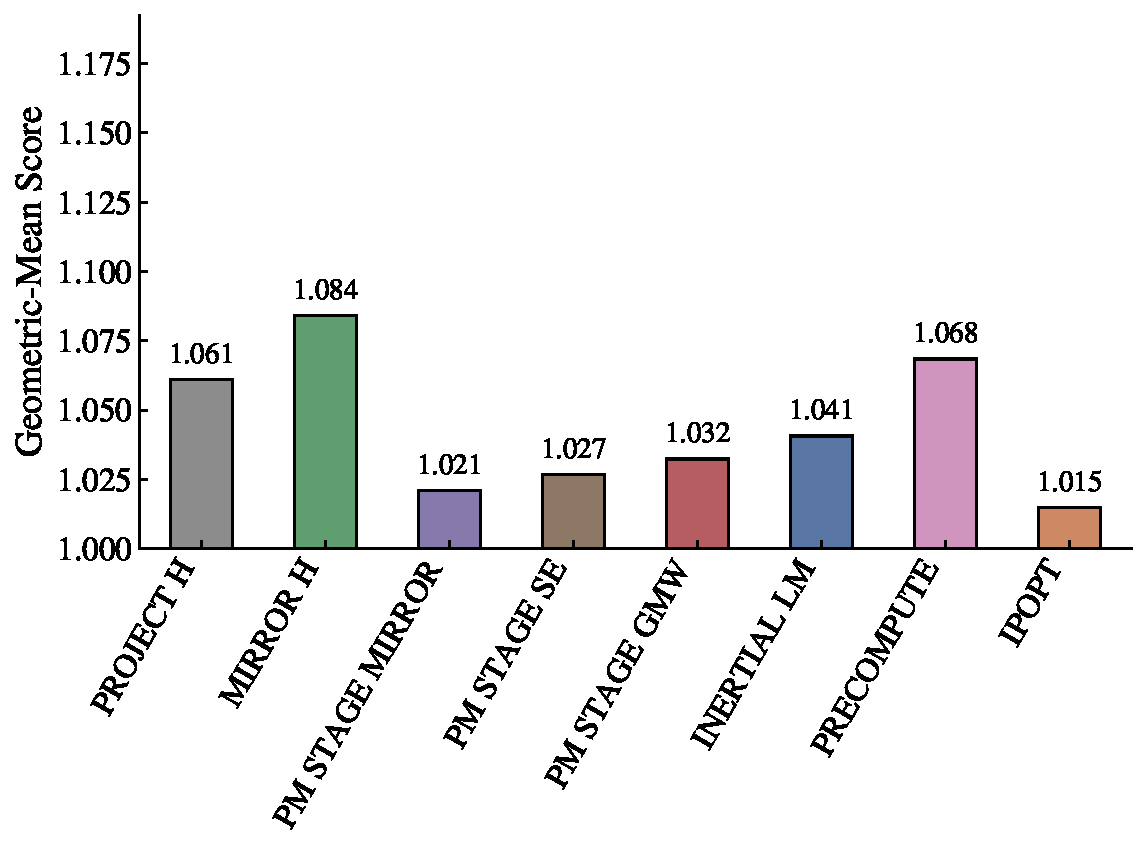
\includegraphics[width=0.70\textwidth]{results/geo_mean_cost_qp_results_riccati.pdf}
    \end{figure}
\end{frame}

\begin{frame}
    \frametitle{Results: box plot of flop count}
    \begin{figure}[H]
        \centering
        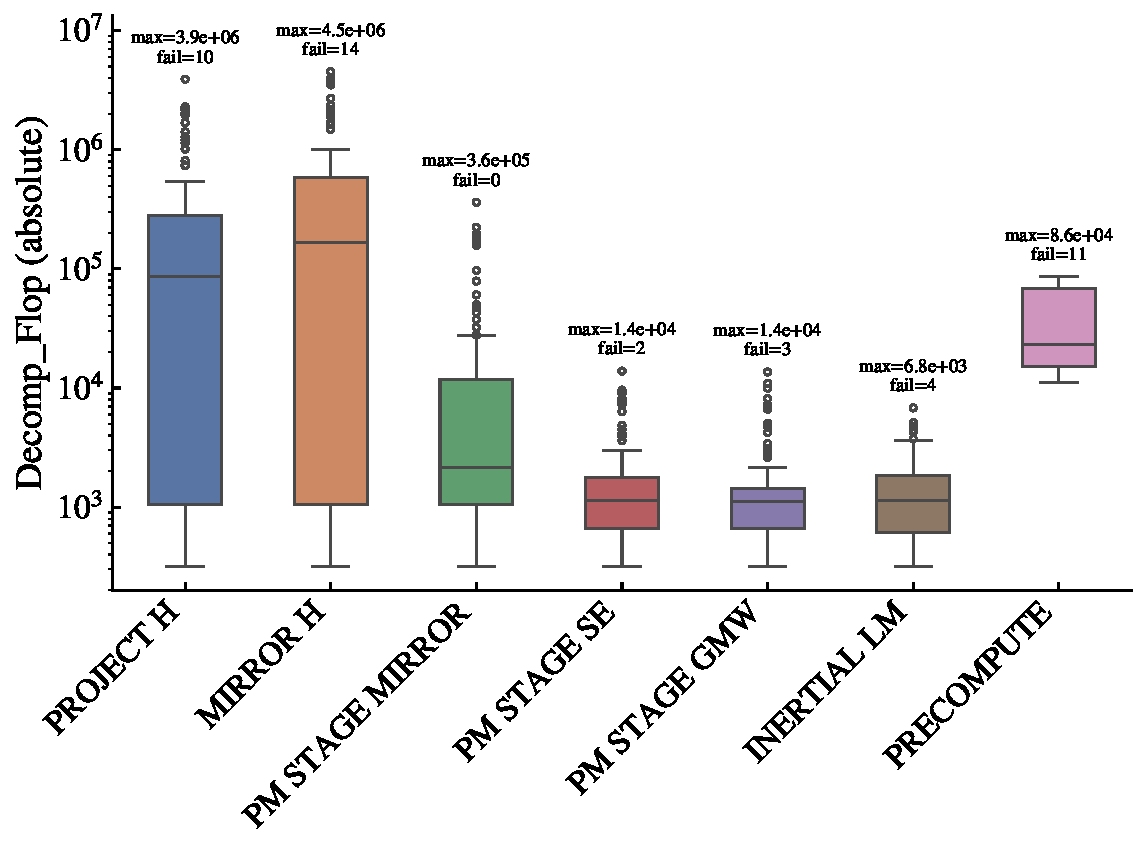
\includegraphics[width=0.70\textwidth]{results/decomp_flop_worstcase_qp_results_riccati.pdf}
    \end{figure}
\end{frame}

\begin{frame}
    \frametitle{Issues and next steps}
    Issue:
    \begin{itemize}
        \item Bad scaling of flops in PM related regularization due to $\mathrm{n}_x^3$
    \end{itemize}
    Next steps:
    \begin{itemize}
        \item More cases for sure, ideal number?
        \item Maybe efficient implementation?
        \item Maybe a native SQP implementation with two-level strategy?:
        \begin{itemize}
            \item first step: solve nonconvex QP subproblem with modified Riccati solver
            \item second step: if first step fails or resulting a too small step length, then convexify the QP subproblem
            \item third step: quickly solve the convexified QP subproblem with Riccati solver, and go back to first step
        \end{itemize}
\end{itemize}

\end{frame}
\bibliographystyle{IEEEtran}
\bibliography{references}

\end{document}
